\documentclass[12pt]{article}

%packages
%\usepackage{latexsym}
\usepackage{graphicx}
\usepackage{color}
\usepackage{amsmath}
\usepackage{dsfont}
\usepackage{placeins}
\usepackage{amssymb}
\usepackage{wasysym}
\usepackage{abstract}
\usepackage{hyperref}
\usepackage{etoolbox}
\usepackage{datetime}
\usepackage{xcolor}
\usepackage{alphalph}
\settimeformat{ampmtime}

%\usepackage{pstricks,pst-node,pst-tree}

%\usepackage{algpseudocode}
%\usepackage{amsthm}
%\usepackage{hyperref}
%\usepackage{mathrsfs}
%\usepackage{amsfonts}
%\usepackage{bbding}
%\usepackage{listings}
%\usepackage{appendix}
\usepackage[margin=1in]{geometry}
%\geometry{papersize={8.5in,11in},total={6.5in,9in}}
%\usepackage{cancel}
%\usepackage{algorithmic, algorithm}

\makeatletter
\def\maxwidth{ %
  \ifdim\Gin@nat@width>\linewidth
    \linewidth
  \else
    \Gin@nat@width
  \fi
}
\makeatother

\definecolor{fgcolor}{rgb}{0.345, 0.345, 0.345}
\newcommand{\hlnum}[1]{\textcolor[rgb]{0.686,0.059,0.569}{#1}}%
\newcommand{\hlstr}[1]{\textcolor[rgb]{0.192,0.494,0.8}{#1}}%
\newcommand{\hlcom}[1]{\textcolor[rgb]{0.678,0.584,0.686}{\textit{#1}}}%
\newcommand{\hlopt}[1]{\textcolor[rgb]{0,0,0}{#1}}%
\newcommand{\hlstd}[1]{\textcolor[rgb]{0.345,0.345,0.345}{#1}}%
\newcommand{\hlkwa}[1]{\textcolor[rgb]{0.161,0.373,0.58}{\textbf{#1}}}%
\newcommand{\hlkwb}[1]{\textcolor[rgb]{0.69,0.353,0.396}{#1}}%
\newcommand{\hlkwc}[1]{\textcolor[rgb]{0.333,0.667,0.333}{#1}}%
\newcommand{\hlkwd}[1]{\textcolor[rgb]{0.737,0.353,0.396}{\textbf{#1}}}%

\usepackage{framed}
\makeatletter
\newenvironment{kframe}{%
 \def\at@end@of@kframe{}%
 \ifinner\ifhmode%
  \def\at@end@of@kframe{\end{minipage}}%
  \begin{minipage}{\columnwidth}%
 \fi\fi%
 \def\FrameCommand##1{\hskip\@totalleftmargin \hskip-\fboxsep
 \colorbox{shadecolor}{##1}\hskip-\fboxsep
     % There is no \\@totalrightmargin, so:
     \hskip-\linewidth \hskip-\@totalleftmargin \hskip\columnwidth}%
 \MakeFramed {\advance\hsize-\width
   \@totalleftmargin\z@ \linewidth\hsize
   \@setminipage}}%
 {\par\unskip\endMakeFramed%
 \at@end@of@kframe}
\makeatother

\definecolor{shadecolor}{rgb}{.77, .77, .77}
\definecolor{messagecolor}{rgb}{0, 0, 0}
\definecolor{warningcolor}{rgb}{1, 0, 1}
\definecolor{errorcolor}{rgb}{1, 0, 0}
\newenvironment{knitrout}{}{} % an empty environment to be redefined in TeX

\usepackage{alltt}
\usepackage[T1]{fontenc}

\newcommand{\qu}[1]{``#1''}
\newcounter{probnum}
\setcounter{probnum}{1}

%create definition to allow local margin changes
\def\changemargin#1#2{\list{}{\rightmargin#2\leftmargin#1}\item[]}
\let\endchangemargin=\endlist 

%allow equations to span multiple pages
\allowdisplaybreaks

%define colors and color typesetting conveniences
\definecolor{gray}{rgb}{0.5,0.5,0.5}
\definecolor{black}{rgb}{0,0,0}
\definecolor{white}{rgb}{1,1,1}
\definecolor{blue}{rgb}{0.5,0.5,1}
\newcommand{\inblue}[1]{\color{blue}#1 \color{black}}
\definecolor{green}{rgb}{0.133,0.545,0.133}
\newcommand{\ingreen}[1]{\color{green}#1 \color{black}}
\definecolor{yellow}{rgb}{1,1,0}
\newcommand{\inyellow}[1]{\color{yellow}#1 \color{black}}
\definecolor{orange}{rgb}{0.9,0.649,0}
\newcommand{\inorange}[1]{\color{orange}#1 \color{black}}
\definecolor{red}{rgb}{1,0.133,0.133}
\newcommand{\inred}[1]{\color{red}#1 \color{black}}
\definecolor{purple}{rgb}{0.58,0,0.827}
\newcommand{\inpurple}[1]{\color{purple}#1 \color{black}}
\definecolor{backgcode}{rgb}{0.97,0.97,0.8}
\definecolor{Brown}{cmyk}{0,0.81,1,0.60}
\definecolor{OliveGreen}{cmyk}{0.64,0,0.95,0.40}
\definecolor{CadetBlue}{cmyk}{0.62,0.57,0.23,0}

%define new math operators
\DeclareMathOperator*{\argmax}{arg\,max~}
\DeclareMathOperator*{\argmin}{arg\,min~}
\DeclareMathOperator*{\argsup}{arg\,sup~}
\DeclareMathOperator*{\arginf}{arg\,inf~}
\DeclareMathOperator*{\convolution}{\text{\Huge{$\ast$}}}
\newcommand{\infconv}[2]{\convolution^\infty_{#1 = 1} #2}
%true functions

%%%% GENERAL SHORTCUTS

%shortcuts for pure typesetting conveniences
\newcommand{\bv}[1]{\boldsymbol{#1}}

%shortcuts for compound constants
\newcommand{\BetaDistrConst}{\dfrac{\Gamma(\alpha + \beta)}{\Gamma(\alpha)\Gamma(\beta)}}
\newcommand{\NormDistrConst}{\dfrac{1}{\sqrt{2\pi\sigma^2}}}

%shortcuts for conventional symbols
\newcommand{\tsq}{\tau^2}
\newcommand{\tsqh}{\hat{\tau}^2}
\newcommand{\sigsq}{\sigma^2}
\newcommand{\sigsqsq}{\parens{\sigma^2}^2}
\newcommand{\sigsqovern}{\dfrac{\sigsq}{n}}
\newcommand{\tausq}{\tau^2}
\newcommand{\tausqalpha}{\tau^2_\alpha}
\newcommand{\tausqbeta}{\tau^2_\beta}
\newcommand{\tausqsigma}{\tau^2_\sigma}
\newcommand{\betasq}{\beta^2}
\newcommand{\sigsqvec}{\bv{\sigma}^2}
\newcommand{\sigsqhat}{\hat{\sigma}^2}
\newcommand{\sigsqhatmlebayes}{\sigsqhat_{\text{Bayes, MLE}}}
\newcommand{\sigsqhatmle}[1]{\sigsqhat_{#1, \text{MLE}}}
\newcommand{\bSigma}{\bv{\Sigma}}
\newcommand{\bSigmainv}{\bSigma^{-1}}
\newcommand{\thetavec}{\bv{\theta}}
\newcommand{\thetahat}{\hat{\theta}}
\newcommand{\thetahatmle}{\hat{\theta}_{\mathrm{MLE}}}
\newcommand{\thetavechatmle}{\hat{\thetavec}_{\mathrm{MLE}}}
\newcommand{\muhat}{\hat{\mu}}
\newcommand{\musq}{\mu^2}
\newcommand{\muvec}{\bv{\mu}}
\newcommand{\muhatmle}{\muhat_{\text{MLE}}}
\newcommand{\lambdahat}{\hat{\lambda}}
\newcommand{\lambdahatmle}{\lambdahat_{\text{MLE}}}
\newcommand{\etavec}{\bv{\eta}}
\newcommand{\alphavec}{\bv{\alpha}}
\newcommand{\minimaxdec}{\delta^*_{\mathrm{mm}}}
\newcommand{\ybar}{\bar{y}}
\newcommand{\xbar}{\bar{x}}
\newcommand{\Xbar}{\bar{X}}
\newcommand{\phat}{\hat{p}}
\newcommand{\Phat}{\hat{P}}
\newcommand{\Zbar}{\bar{Z}}
\newcommand{\iid}{~{\buildrel iid \over \sim}~}
\newcommand{\inddist}{~{\buildrel ind \over \sim}~}
\newcommand{\approxdist}{~{\buildrel approx \over \sim}~}
\newcommand{\equalsindist}{~{\buildrel d \over =}~}
\newcommand{\loglik}[1]{\ell\parens{#1}}
\newcommand{\thetahatkminone}{\thetahat^{(k-1)}}
\newcommand{\thetahatkplusone}{\thetahat^{(k+1)}}
\newcommand{\thetahatk}{\thetahat^{(k)}}
\newcommand{\half}{\frac{1}{2}}
\newcommand{\third}{\frac{1}{3}}
\newcommand{\twothirds}{\frac{2}{3}}
\newcommand{\fourth}{\frac{1}{4}}
\newcommand{\fifth}{\frac{1}{5}}
\newcommand{\sixth}{\frac{1}{6}}

%shortcuts for vector and matrix notation
\newcommand{\A}{\bv{A}}
\newcommand{\At}{\A^T}
\newcommand{\Ainv}{\inverse{\A}}
\newcommand{\B}{\bv{B}}
\newcommand{\K}{\bv{K}}
\newcommand{\Kt}{\K^T}
\newcommand{\Kinv}{\inverse{K}}
\newcommand{\Kinvt}{(\Kinv)^T}
\newcommand{\M}{\bv{M}}
\newcommand{\Bt}{\B^T}
\newcommand{\Q}{\bv{Q}}
\newcommand{\Qt}{\Q^T}
\newcommand{\R}{\bv{R}}
\newcommand{\Rt}{\R^T}
\newcommand{\Z}{\bv{Z}}
\newcommand{\X}{\bv{X}}
\newcommand{\Xsub}{\X_{\text{(sub)}}}
\newcommand{\Xsubadj}{\X_{\text{(sub,adj)}}}
\newcommand{\I}{\bv{I}}
\newcommand{\Y}{\bv{Y}}
\newcommand{\sigsqI}{\sigsq\I}
\renewcommand{\P}{\bv{P}}
\newcommand{\Psub}{\P_{\text{(sub)}}}
\newcommand{\Pt}{\P^T}
\newcommand{\Pii}{P_{ii}}
\newcommand{\Pij}{P_{ij}}
\newcommand{\IminP}{(\I-\P)}
\newcommand{\Xt}{\bv{X}^T}
\newcommand{\XtX}{\Xt\X}
\newcommand{\XtXinv}{\parens{\Xt\X}^{-1}}
\newcommand{\XtXinvXt}{\XtXinv\Xt}
\newcommand{\XXtXinvXt}{\X\XtXinvXt}
\newcommand{\x}{\bv{x}}
\newcommand{\onevec}{\bv{1}}
\newcommand{\oneton}{1, \ldots, n}
\newcommand{\yoneton}{y_1, \ldots, y_n}
\newcommand{\yonetonorder}{y_{(1)}, \ldots, y_{(n)}}
\newcommand{\Yoneton}{Y_1, \ldots, Y_n}
\newcommand{\iinoneton}{i \in \braces{\oneton}}
\newcommand{\onetom}{1, \ldots, m}
\newcommand{\jinonetom}{j \in \braces{\onetom}}
\newcommand{\xoneton}{x_1, \ldots, x_n}
\newcommand{\Xoneton}{X_1, \ldots, X_n}
\newcommand{\xt}{\x^T}
\newcommand{\y}{\bv{y}}
\newcommand{\yt}{\y^T}
\renewcommand{\c}{\bv{c}}
\newcommand{\ct}{\c^T}
\newcommand{\tstar}{\bv{t}^*}
\renewcommand{\u}{\bv{u}}
\renewcommand{\v}{\bv{v}}
\renewcommand{\a}{\bv{a}}
\newcommand{\s}{\bv{s}}
\newcommand{\yadj}{\y_{\text{(adj)}}}
\newcommand{\xjadj}{\x_{j\text{(adj)}}}
\newcommand{\xjadjM}{\x_{j \perp M}}
\newcommand{\yhat}{\hat{\y}}
\newcommand{\yhatsub}{\yhat_{\text{(sub)}}}
\newcommand{\yhatstar}{\yhat^*}
\newcommand{\yhatstarnew}{\yhatstar_{\text{new}}}
\newcommand{\z}{\bv{z}}
\newcommand{\zt}{\z^T}
\newcommand{\bb}{\bv{b}}
\newcommand{\bbt}{\bb^T}
\newcommand{\bbeta}{\bv{\beta}}
\newcommand{\beps}{\bv{\epsilon}}
\newcommand{\bepst}{\beps^T}
\newcommand{\e}{\bv{e}}
\newcommand{\Mofy}{\M(\y)}
\newcommand{\KofAlpha}{K(\alpha)}
\newcommand{\ellset}{\mathcal{L}}
\newcommand{\oneminalph}{1-\alpha}
\newcommand{\SSE}{\text{SSE}}
\newcommand{\SSEsub}{\text{SSE}_{\text{(sub)}}}
\newcommand{\MSE}{\text{MSE}}
\newcommand{\RMSE}{\text{RMSE}}
\newcommand{\SSR}{\text{SSR}}
\newcommand{\SST}{\text{SST}}
\newcommand{\JSest}{\delta_{\text{JS}}(\x)}
\newcommand{\Bayesest}{\delta_{\text{Bayes}}(\x)}
\newcommand{\EmpBayesest}{\delta_{\text{EmpBayes}}(\x)}
\newcommand{\BLUPest}{\delta_{\text{BLUP}}}
\newcommand{\MLEest}[1]{\hat{#1}_{\text{MLE}}}

%shortcuts for Linear Algebra stuff (i.e. vectors and matrices)
\newcommand{\twovec}[2]{\bracks{\begin{array}{c} #1 \\ #2 \end{array}}}
\newcommand{\threevec}[3]{\bracks{\begin{array}{c} #1 \\ #2 \\ #3 \end{array}}}
\newcommand{\fivevec}[5]{\bracks{\begin{array}{c} #1 \\ #2 \\ #3 \\ #4 \\ #5 \end{array}}}
\newcommand{\twobytwomat}[4]{\bracks{\begin{array}{cc} #1 & #2 \\ #3 & #4 \end{array}}}
\newcommand{\threebytwomat}[6]{\bracks{\begin{array}{cc} #1 & #2 \\ #3 & #4 \\ #5 & #6 \end{array}}}

%shortcuts for conventional compound symbols
\newcommand{\thetainthetas}{\theta \in \Theta}
\newcommand{\reals}{\mathbb{R}}
\newcommand{\complexes}{\mathbb{C}}
\newcommand{\rationals}{\mathbb{Q}}
\newcommand{\integers}{\mathbb{Z}}
\newcommand{\naturals}{\mathbb{N}}
\newcommand{\forallninN}{~~\forall n \in \naturals}
\newcommand{\forallxinN}[1]{~~\forall #1 \in \reals}
\newcommand{\matrixdims}[2]{\in \reals^{\,#1 \times #2}}
\newcommand{\inRn}[1]{\in \reals^{\,#1}}
\newcommand{\mathimplies}{\quad\Rightarrow\quad}
\newcommand{\mathlogicequiv}{\quad\Leftrightarrow\quad}
\newcommand{\eqncomment}[1]{\quad \text{(#1)}}
\newcommand{\limitn}{\lim_{n \rightarrow \infty}}
\newcommand{\limitN}{\lim_{N \rightarrow \infty}}
\newcommand{\limitd}{\lim_{d \rightarrow \infty}}
\newcommand{\limitt}{\lim_{t \rightarrow \infty}}
\newcommand{\limitsupn}{\limsup_{n \rightarrow \infty}~}
\newcommand{\limitinfn}{\liminf_{n \rightarrow \infty}~}
\newcommand{\limitk}{\lim_{k \rightarrow \infty}}
\newcommand{\limsupn}{\limsup_{n \rightarrow \infty}}
\newcommand{\limsupk}{\limsup_{k \rightarrow \infty}}
\newcommand{\floor}[1]{\left\lfloor #1 \right\rfloor}
\newcommand{\ceil}[1]{\left\lceil #1 \right\rceil}

%shortcuts for environments
\newcommand{\beqn}{\vspace{-0.25cm}\begin{eqnarray*}}
\newcommand{\eeqn}{\end{eqnarray*}}
\newcommand{\bneqn}{\vspace{-0.25cm}\begin{eqnarray}}
\newcommand{\eneqn}{\end{eqnarray}}

%shortcuts for mini environments
\newcommand{\parens}[1]{\left(#1\right)}
\newcommand{\squared}[1]{\parens{#1}^2}
\newcommand{\tothepow}[2]{\parens{#1}^{#2}}
\newcommand{\prob}[1]{\mathbb{P}\parens{#1}}
\newcommand{\cprob}[2]{\prob{#1~|~#2}}
\newcommand{\littleo}[1]{o\parens{#1}}
\newcommand{\bigo}[1]{O\parens{#1}}
\newcommand{\Lp}[1]{\mathbb{L}^{#1}}
\renewcommand{\arcsin}[1]{\text{arcsin}\parens{#1}}
\newcommand{\prodonen}[2]{\bracks{\prod_{#1=1}^n #2}}
\newcommand{\mysum}[4]{\sum_{#1=#2}^{#3} #4}
\newcommand{\sumonen}[2]{\sum_{#1=1}^n #2}
\newcommand{\infsum}[2]{\sum_{#1=1}^\infty #2}
\newcommand{\infprod}[2]{\prod_{#1=1}^\infty #2}
\newcommand{\infunion}[2]{\bigcup_{#1=1}^\infty #2}
\newcommand{\infinter}[2]{\bigcap_{#1=1}^\infty #2}
\newcommand{\infintegral}[2]{\int^\infty_{-\infty} #2 ~\text{d}#1}
\newcommand{\supthetas}[1]{\sup_{\thetainthetas}\braces{#1}}
\newcommand{\bracks}[1]{\left[#1\right]}
\newcommand{\braces}[1]{\left\{#1\right\}}
\newcommand{\angbraces}[1]{\left<#1\right>}
\newcommand{\set}[1]{\left\{#1\right\}}
\newcommand{\abss}[1]{\left|#1\right|}
\newcommand{\norm}[1]{\left|\left|#1\right|\right|}
\newcommand{\normsq}[1]{\norm{#1}^2}
\newcommand{\inverse}[1]{\parens{#1}^{-1}}
\newcommand{\rowof}[2]{\parens{#1}_{#2\cdot}}

%shortcuts for functionals
\newcommand{\realcomp}[1]{\text{Re}\bracks{#1}}
\newcommand{\imagcomp}[1]{\text{Im}\bracks{#1}}
\newcommand{\range}[1]{\text{range}\bracks{#1}}
\newcommand{\colsp}[1]{\text{colsp}\bracks{#1}}
\newcommand{\rowsp}[1]{\text{rowsp}\bracks{#1}}
\newcommand{\tr}[1]{\text{tr}\bracks{#1}}
\newcommand{\rank}[1]{\text{rank}\bracks{#1}}
\newcommand{\proj}[2]{\text{Proj}_{#1}\bracks{#2}}
\newcommand{\projcolspX}[1]{\text{Proj}_{\colsp{\X}}\bracks{#1}}
\newcommand{\median}[1]{\text{median}\bracks{#1}}
\newcommand{\mean}[1]{\text{mean}\bracks{#1}}
\newcommand{\dime}[1]{\text{dim}\bracks{#1}}
\renewcommand{\det}[1]{\text{det}\bracks{#1}}
\newcommand{\expe}[1]{\mathbb{E}\bracks{#1}}
\newcommand{\expeabs}[1]{\expe{\abss{#1}}}
\newcommand{\expesub}[2]{\mathbb{E}_{#1}\bracks{#2}}
\newcommand{\indic}[1]{\mathds{1}_{#1}}
\newcommand{\var}[1]{\mathbb{V}\text{ar}\bracks{#1}}
\newcommand{\cov}[2]{\mathbb{C}\text{ov}\bracks{#1, #2}}
\newcommand{\corr}[2]{\text{Corr}\bracks{#1, #2}}
\newcommand{\se}[1]{\mathbb{S}\text{E}\bracks{#1}}
\newcommand{\seest}[1]{\hat{\text{SE}}\bracks{#1}}
\newcommand{\bias}[1]{\text{Bias}\bracks{#1}}
\newcommand{\derivop}[2]{\dfrac{\text{d}}{\text{d} #1}\bracks{#2}}
\newcommand{\partialop}[2]{\dfrac{\partial}{\partial #1}\bracks{#2}}
\newcommand{\secpartialop}[2]{\dfrac{\partial^2}{\partial #1^2}\bracks{#2}}
\newcommand{\mixpartialop}[3]{\dfrac{\partial^2}{\partial #1 \partial #2}\bracks{#3}}

%shortcuts for functions
\renewcommand{\exp}[1]{\mathrm{exp}\parens{#1}}
\renewcommand{\cos}[1]{\text{cos}\parens{#1}}
\renewcommand{\sin}[1]{\text{sin}\parens{#1}}
\newcommand{\sign}[1]{\text{sign}\parens{#1}}
\newcommand{\are}[1]{\mathrm{ARE}\parens{#1}}
\newcommand{\natlog}[1]{\ln\parens{#1}}
\newcommand{\oneover}[1]{\frac{1}{#1}}
\newcommand{\overtwo}[1]{\frac{#1}{2}}
\newcommand{\overn}[1]{\frac{#1}{n}}
\newcommand{\oneoversqrt}[1]{\oneover{\sqrt{#1}}}
\newcommand{\sqd}[1]{\parens{#1}^2}
\newcommand{\loss}[1]{\ell\parens{\theta, #1}}
\newcommand{\losstwo}[2]{\ell\parens{#1, #2}}
\newcommand{\cf}{\phi(t)}

%English language specific shortcuts
\newcommand{\ie}{\textit{i.e.} }
\newcommand{\AKA}{\textit{AKA} }
\renewcommand{\iff}{\textit{iff}}
\newcommand{\eg}{\textit{e.g.} }
\newcommand{\st}{\textit{s.t.} }
\newcommand{\wrt}{\textit{w.r.t.} }
\newcommand{\mathst}{~~\text{\st}~~}
\newcommand{\mathand}{~~\text{and}~~}
\newcommand{\ala}{\textit{a la} }
\newcommand{\ppp}{posterior predictive p-value}
\newcommand{\dd}{dataset-to-dataset}

%shortcuts for distribution titles
\newcommand{\logistic}[2]{\mathrm{Logistic}\parens{#1,\,#2}}
\newcommand{\bernoulli}[1]{\mathrm{Bernoulli}\parens{#1}}
\newcommand{\betanot}[2]{\mathrm{Beta}\parens{#1,\,#2}}
\newcommand{\stdbetanot}{\betanot{\alpha}{\beta}}
\newcommand{\multnormnot}[3]{\mathcal{N}_{#1}\parens{#2,\,#3}}
\newcommand{\normnot}[2]{\mathcal{N}\parens{#1,\,#2}}
\newcommand{\classicnormnot}{\normnot{\mu}{\sigsq}}
\newcommand{\stdnormnot}{\normnot{0}{1}}
\newcommand{\uniformdiscrete}[1]{\mathrm{Uniform}\parens{\braces{#1}}}
\newcommand{\uniform}[2]{\mathrm{U}\parens{#1,\,#2}}
\newcommand{\stduniform}{\uniform{0}{1}}
\newcommand{\geometric}[1]{\mathrm{Geometric}\parens{#1}}
\newcommand{\hypergeometric}[3]{\mathrm{Hypergeometric}\parens{#1,\,#2,\,#3}}
\newcommand{\exponential}[1]{\mathrm{Exp}\parens{#1}}
\newcommand{\gammadist}[2]{\mathrm{Gamma}\parens{#1, #2}}
\newcommand{\poisson}[1]{\mathrm{Poisson}\parens{#1}}
\newcommand{\binomial}[2]{\mathrm{Binomial}\parens{#1,\,#2}}
\newcommand{\negbin}[2]{\mathrm{NegBin}\parens{#1,\,#2}}
\newcommand{\rayleigh}[1]{\mathrm{Rayleigh}\parens{#1}}
\newcommand{\multinomial}[2]{\mathrm{Multinomial}\parens{#1,\,#2}}
\newcommand{\gammanot}[2]{\mathrm{Gamma}\parens{#1,\,#2}}
\newcommand{\cauchynot}[2]{\text{Cauchy}\parens{#1,\,#2}}
\newcommand{\invchisqnot}[1]{\text{Inv}\chisq{#1}}
\newcommand{\invscaledchisqnot}[2]{\text{ScaledInv}\ncchisq{#1}{#2}}
\newcommand{\invgammanot}[2]{\text{InvGamma}\parens{#1,\,#2}}
\newcommand{\chisq}[1]{\chi^2_{#1}}
\newcommand{\ncchisq}[2]{\chi^2_{#1}\parens{#2}}
\newcommand{\ncF}[3]{F_{#1,#2}\parens{#3}}

%shortcuts for PDF's of common distributions
\newcommand{\logisticpdf}[3]{\oneover{#3}\dfrac{\exp{-\dfrac{#1 - #2}{#3}}}{\parens{1+\exp{-\dfrac{#1 - #2}{#3}}}^2}}
\newcommand{\betapdf}[3]{\dfrac{\Gamma(#2 + #3)}{\Gamma(#2)\Gamma(#3)}#1^{#2-1} (1-#1)^{#3-1}}
\newcommand{\normpdf}[3]{\frac{1}{\sqrt{2\pi#3}}\exp{-\frac{1}{2#3}(#1 - #2)^2}}
\newcommand{\normpdfvarone}[2]{\dfrac{1}{\sqrt{2\pi}}e^{-\half(#1 - #2)^2}}
\newcommand{\chisqpdf}[2]{\dfrac{1}{2^{#2/2}\Gamma(#2/2)}\; {#1}^{#2/2-1} e^{-#1/2}}
\newcommand{\invchisqpdf}[2]{\dfrac{2^{-\overtwo{#1}}}{\Gamma(#2/2)}\,{#1}^{-\overtwo{#2}-1}  e^{-\oneover{2 #1}}}
\newcommand{\exponentialpdf}[2]{#2\exp{-#2#1}}
\newcommand{\poissonpdf}[2]{\dfrac{e^{-#1} #1^{#2}}{#2!}}
\newcommand{\binomialpdf}[3]{\binom{#2}{#1}#3^{#1}(1-#3)^{#2-#1}}
\newcommand{\rayleighpdf}[2]{\dfrac{#1}{#2^2}\exp{-\dfrac{#1^2}{2 #2^2}}}
\newcommand{\gammapdf}[3]{\dfrac{#3^#2}{\Gamma\parens{#2}}#1^{#2-1}\exp{-#3 #1}}
\newcommand{\cauchypdf}[3]{\oneover{\pi} \dfrac{#3}{\parens{#1-#2}^2 + #3^2}}
\newcommand{\Gammaf}[1]{\Gamma\parens{#1}}

%shortcuts for miscellaneous typesetting conveniences
\newcommand{\notesref}[1]{\marginpar{\color{gray}\tt #1\color{black}}}

%%%% DOMAIN-SPECIFIC SHORTCUTS

%Real analysis related shortcuts
\newcommand{\zeroonecl}{\bracks{0,1}}
\newcommand{\forallepsgrzero}{\forall \epsilon > 0~~}
\newcommand{\lessthaneps}{< \epsilon}
\newcommand{\fraccomp}[1]{\text{frac}\bracks{#1}}

%Bayesian related shortcuts
\newcommand{\yrep}{y^{\text{rep}}}
\newcommand{\yrepisq}{(\yrep_i)^2}
\newcommand{\yrepvec}{\bv{y}^{\text{rep}}}


%Probability shortcuts
\newcommand{\SigField}{\mathcal{F}}
\newcommand{\ProbMap}{\mathcal{P}}
\newcommand{\probtrinity}{\parens{\Omega, \SigField, \ProbMap}}
\newcommand{\convp}{~{\buildrel p \over \rightarrow}~}
\newcommand{\convLp}[1]{~{\buildrel \Lp{#1} \over \rightarrow}~}
\newcommand{\nconvp}{~{\buildrel p \over \nrightarrow}~}
\newcommand{\convae}{~{\buildrel a.e. \over \longrightarrow}~}
\newcommand{\convau}{~{\buildrel a.u. \over \longrightarrow}~}
\newcommand{\nconvau}{~{\buildrel a.u. \over \nrightarrow}~}
\newcommand{\nconvae}{~{\buildrel a.e. \over \nrightarrow}~}
\newcommand{\convd}{~{\buildrel \mathcal{D} \over \rightarrow}~}
\newcommand{\nconvd}{~{\buildrel \mathcal{D} \over \nrightarrow}~}
\newcommand{\withprob}{~~\text{w.p.}~~}
\newcommand{\io}{~~\text{i.o.}}

\newcommand{\Acl}{\bar{A}}
\newcommand{\ENcl}{\bar{E}_N}
\newcommand{\diam}[1]{\text{diam}\parens{#1}}

\newcommand{\taua}{\tau_a}

\newcommand{\myint}[4]{\int_{#2}^{#3} #4 \,\text{d}#1}
\newcommand{\laplacet}[1]{\mathscr{L}\bracks{#1}}
\newcommand{\laplaceinvt}[1]{\mathscr{L}^{-1}\bracks{#1}}
\renewcommand{\min}[1]{\text{min}\braces{#1}}
\renewcommand{\max}[1]{\text{max}\braces{#1}}

\newcommand{\Vbar}[1]{\bar{V}\parens{#1}}
\newcommand{\expnegrtau}{\exp{-r\tau}}

%%% problem typesetting
\newcommand{\problem}{\noindent \colorbox{black}{{\color{yellow} \large{\textsf{\textbf{Problem \arabic{probnum}}}}~}} \addtocounter{probnum}{1} \vspace{0.2cm} \\ }

\newcommand{\easysubproblem}{\ingreen{\item} [easy] }
\newcommand{\intermediatesubproblem}{\inorange{\item} [harder] }
\newcommand{\hardsubproblem}{\inred{\item} [difficult] }
\newcommand{\extracreditsubproblem}{\inpurple{\item} [E.C.] }

\makeatletter
\newalphalph{\alphmult}[mult]{\@alph}{26}
\renewcommand{\labelenumi}{(\alphmult{\value{enumi}})}

\newcommand{\support}[1]{\text{Supp}\bracks{#1}}
\newcommand{\mode}[1]{\text{Mode}\bracks{#1}}
\newcommand{\IQR}[1]{\text{IQR}\bracks{#1}}
\newcommand{\quantile}[2]{\text{Quantile}\bracks{#1,\,#2}}


\newtoggle{professormode}
\toggletrue{professormode} %STUDENTS: DELETE or COMMENT this line



\title{MATH 241 Fall 2017 Homework \#4}

\author{Professor Adam Kapelner} %STUDENTS: write your name here

\iftoggle{professormode}{
\date{Due 8PM KY604 (under door) or in the review session to me or TA (KY150), \\ Monday, November 13, 2017 \\ \vspace{0.5cm} \small (this document last updated \today ~at \currenttime)}
}

\renewcommand{\abstractname}{Instructions and Philosophy}




\begin{document}
\maketitle

\iftoggle{professormode}{
\begin{abstract}
The path to success in this class is to do many problems. Unlike other courses, exclusively doing reading(s) will not help. Coming to lecture is akin to watching workout videos; thinking about and solving problems on your own is the actual ``working out''.  Feel free to \qu{work out} with others; \textbf{I want you to work on this in groups.}

Reading is still \textit{required}. For this homework set, read the section about discrete random variables especially the Bernoulli, the Binomial and the Geometric.

The problems below are color coded: \ingreen{green} problems are considered \textit{easy} and marked \qu{[easy]}; \inorange{yellow} problems are considered \textit{intermediate} and marked \qu{[harder]}, \inred{red} problems are considered \textit{difficult} and marked \qu{[difficult]} and \inpurple{purple} problems are extra credit. The \textit{easy} problems are intended to be ``giveaways'' if you went to class. Do as much as you can of the others; I expect you to at least attempt the \textit{difficult} problems.

This homework is worth 100 points but the point distribution will not be determined until after the due date. See syllabus for the policy on late homework.

Up to 15 points are given as a bonus if the homework is typed using \LaTeX. Links to instaling \LaTeX~and program for compiling \LaTeX~is found on the syllabus. You are encouraged to use \url{overleaf.com}. If you are handing in homework this way, upload \texttt{hwxx.tex} and \texttt{preamble.tex}, read the comments in the code; there are two lines to comment out and you should replace my name with yours and write your section. If you are asked to make drawings, you can take a picture of your handwritten drawing and insert them as figures or leave space using the \qu{$\backslash$vspace} command and draw them in after printing or attach them stapled.

The document is available with spaces for you to write your answers. If not using \LaTeX, print this document and write in your answers. I do not accept homeworks not on this printout. Keep this first page printed for your records. Write your name and section below (A, B or C).

\end{abstract}

\thispagestyle{empty}
\vspace{1cm}
NAME: \line(1,0){220} ~~SECTION (A, B or C): \line(1,0){35}
\vspace{2cm}\clearpage
}

\problem{Imagine you are flipping the same bundle of coins from the practice midterm. The probability of the coin bundle landing on its side is $\prob{S} = 1/11$. Heads and tail probability are 5/11. Let's call landing on its side a \qu{success.}}

\iftoggle{professormode}{
\begin{figure}[htp]
\centering
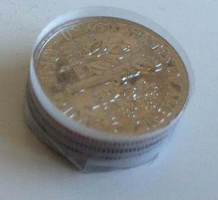
\includegraphics[width=1.5in]{coins.png}
\end{figure}
\FloatBarrier
}

\begin{enumerate}

\easysubproblem{I flip the coin bundle once. Model a success as a \qu{1.} Show that the r.v. modeling this event outcome is Bernoulli and define its parameter.  Write \qu{$X \sim$} something below. }\spc{2}

\easysubproblem{Let's say we flip 10 times. What is the probability that we get one (and only one) success? I want to see a probability model.  Write \qu{$X \sim$} something below. Then I want to see a probability statement. Then I want to see a computation. Answer then in decimal rounded to two digits.  }\spc{3}

\easysubproblem{Let's say we flip 10 times. What is the probability that we get 5 (and only 5) successes? }\spc{3}

\easysubproblem{Let's say we flip 10 times. What is the probability that we get 8 (and only 8) successes? }\spc{3}

\intermediatesubproblem{ Let's say we flip 10 times. What is the probability we get one or two successes? }\spc{3}

\hardsubproblem{ Let's say we flip 10 times. What is the probability we get 3 or less successes?}\spc{3}

\end{enumerate}

\problem{Now that we understand both the binomial and the concept of $\iid$, we will ask some conceptual questions.}

\begin{enumerate}


\intermediatesubproblem{ The human mouth has 32 teeth. If the probability of a cavity at some point in a lifetime is 5\%, is it possible to calculate the probability of 7 cavities during a lifetime using a binomial r.v. model $X \sim \binomial{32}{5\%}$ and computing $\prob{X=7}$? Why or why not?  }\spc{4}

\intermediatesubproblem{Bob drives his car twice a day during the workweek, 50 weeks per year for a total of 200 work days and thus, 400 commuting rides. If the probability of getting into an accident is about 1/1000, could we say the number of accidents per year can be modeled as a r.v. $X \sim \binomial{400}{1/1000}$? Why or why not?}\spc{6}

\end{enumerate}


\problem{We will be investigating r.v.'s by imagining a trip the grocery store to buy ingredients for guacamole.

\iftoggle{professormode}{
\begin{figure}[htp]
\centering
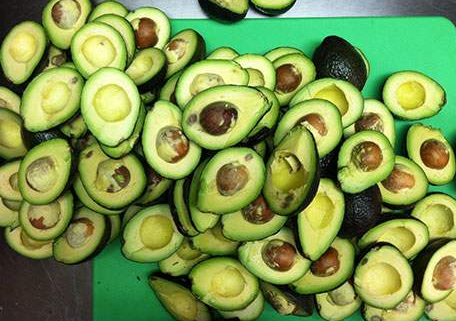
\includegraphics[width=2.5in]{avocados.png}
\end{figure}
\FloatBarrier
}}

\begin{enumerate}

\easysubproblem{You buy \textit{one} avocado at the grocery store which is good (c.f. a bad avocado which may have brown inside because it's partially rotten). Call this probability of good $p$. Model the number of \textit{good} avocados you have using a random variable. All you need to write is $X \sim$ something. You do not need to write the PMF, draw the PMF, draw the CDF, etc. }\spc{0.5}


\hardsubproblem{You take one avocado, cut it open and see if it's rotten. You keep doing this until you see a \textit{rotten} avocado. Model the number of avocados you cut open using a r.v. Call this r.v. $X$. Be careful between \qu{rotten} and \qu{good}.}\spc{1}

\easysubproblem{Write the PMF for the r.v. you created in (b).  }\spc{1}

\easysubproblem{Write the support for the r.v. you created in (b).  }\spc{1}

\easysubproblem{What is the probability you stop when looking at the third avocado?  }\spc{1}

\easysubproblem{Use the sigma notation for summing (e.g. $\sum_{i=1}^5$) to calculate the probability that you stop between 4 and 37 avocados (including 4 and including 37). Since you don't know $p$ you cannot actually compute a numerical value for this probability. Leave it in sigma notation.  }\spc{1}


\intermediatesubproblem{Let's say at some point in your avocado shopping that you learned how to detect rotten avocadoes by using the \qu{squeeze test} and you used this learning to select new avocados. What assumption(s) would be violated?  }\spc{2}

\intermediatesubproblem{Grocery stores usually put the old avocados on the top of the avocado basked and thus the new avocados on the bottom. If your strategy was just to pick the \qu{top} avocado each time, what assumption(s) would be violated?}\spc{2}

\end{enumerate}


\problem{Some simple definitional questions.}

\begin{enumerate}

\easysubproblem{What is a realization of a r.v.?}\spc{4}

\easysubproblem{Define \qu{datum}.}\spc{1}

\easysubproblem{Define \qu{data}.}\spc{1}

\easysubproblem{In a given r.v. model $X$, what set do they data belong to?}\spc{1}

\easysubproblem{Define \qu{iid data}.}\spc{2}

\end{enumerate}


\problem{This is the fun part of the homework. You're going to repeat the experiments we did in class. Let's make some data!

\iftoggle{professormode}{
\begin{figure}[htp]
\centering

\includegraphics[width=3in]{magic.jpg}
\end{figure}
\FloatBarrier
}}

\begin{enumerate}

\easysubproblem{Grab a cup and 8 pennies (or nickels, or dimes, etc). Use a magic marker to mark four of them (front and back). If you shake the cup and pull out three coins, let $X$ be the r.v. for how many marked coins you pull out? How is $X$ distributed? Write \qu{$X \sim$ something} below.}\spc{1}

\easysubproblem{Using as fact that $\expe{X} = n\frac{K}{N}$ when  $X \sim \hypergeometric{n}{K}{N}$ (see Problem 6), calculate $\expe{X}$ for the r.v. you constructed in part (a). }\spc{3}

\easysubproblem{Shake the cup and take out 3 coins. How many were marked? Repeat this five times. 
Record your data below. That is, just write down the five numbers separated by commas.}\spc{1}

\easysubproblem{Find $\xbar$ from the data you recorded in part (c). }\spc{0.5}

\easysubproblem{Is $\xbar \approx \expe{X}$? If not, what could you change in the experiment to make $\xbar$ closer to $\expe{X}$? }\spc{1}

\easysubproblem{Now forget that the coins are marked. If you shake the cup and flip all 8 coins, let $X$ be the r.v. for how many heads are flipped. How is $X$ distributed? Write \qu{$X \sim$ something} below.}\spc{1}

\easysubproblem{Using the fact we proved in class that $\expe{X} = np$ when $X \sim \binomial{n}{p}$, calculate $\expe{X}$ for the r.v. you constructed in part (f). }\spc{1}

\easysubproblem{Shake the cup and count the number of heads. Repeat this five times. 
Record your data below. }\spc{1}

\easysubproblem{Find $\xbar$ from the data you recorded in part (h).  }\spc{0.5}

\easysubproblem{Is $\xbar \approx \expe{X}$? If not, what could you change in the experiment to make $\xbar$ closer to $\expe{X}$? }\spc{1}


\easysubproblem{Now imagine one coin in the cup and success is defined as getting a head. Further imagine that you don't stop flipping this coin until you get a head. Let $X$ be the r.v. for how many flips you make. How is $X$ distributed? Write \qu{$X \sim$ something} below. }\spc{1}

\easysubproblem{Using the fact we proved in class that $\expe{X} = 1/p$ when  $X \sim \geometric{p}$, calculate $\expe{X}$ for the r.v. you constructed in part (k). }\spc{1}

\easysubproblem{Flip until you get a head. Repeat this five times. Record your data below. }\spc{1}

\easysubproblem{Find $\xbar$ from the data you recorded in part (m).  }\spc{0.5}

\easysubproblem{Is $\xbar \approx \expe{X}$? If not, what could you change in the experiment to make $\xbar$ closer to $\expe{X}$? }\spc{1}

\extracreditsubproblem{$X \sim \hypergeometric{n}{K}{N}$. Verify $\expe{X} = n\frac{K}{N}$ from the definition of $\expe{X}$.}\spc{9}
 
\end{enumerate}


\problem{We are going to return to our in-class discussion of the my ride from QC to Forest Hills using the Uber Taxi service. Since Queens is in New York City, I will be modeling based on Uber NYC rates. Some numbers have changed from our in-class discussion.

\iftoggle{professormode}{
\begin{figure}[htp]
\centering
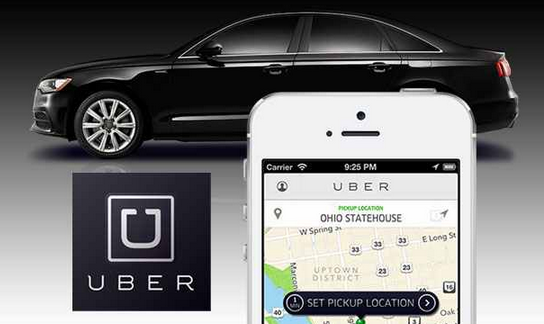
\includegraphics[width=2.5in]{uber.png}
\end{figure}
\FloatBarrier
}

\noindent For the purposes of this exercise, assume there are only two routes in which to drive back. This is close to realistic. There is the \qu{Van Wyck} (outlined in black on the right below) and \qu{Jewel Ave} which is the Q64 bus route (outlined in black on the left below).

\iftoggle{professormode}{
\begin{figure}[htp]
\centering
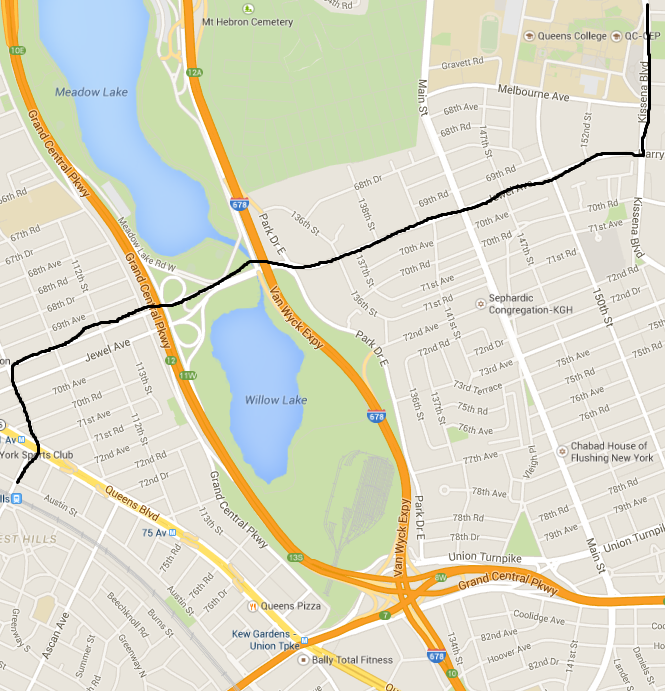
\includegraphics[width=3in]{route1.png}~~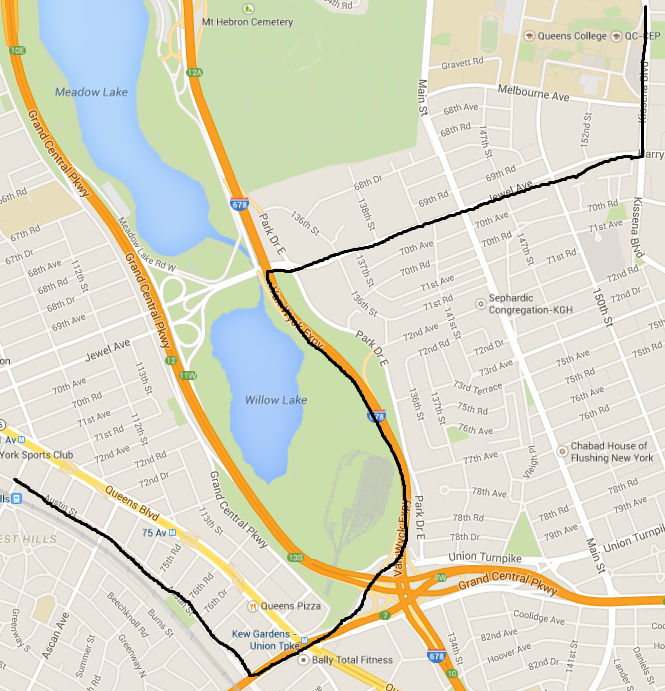
\includegraphics[width=3in]{route2.png}
\end{figure}
\FloatBarrier
}

\noindent The only determinant of route selection is whether or not there is traffic on the Van Wyck. If there is traffic, I take Jewel Ave route; if not, I take the Van Wyck route. The probability of traffic on the Van Wyck is 30\%. The Jewel Ave route is 2.3 miles and takes 13 min and the Van Wyck route is 8 min and is 3.6 miles.}

\begin{enumerate}
\easysubproblem{Let $W$ be the r.v. which models the time I travel in the Uber Taxi. What is its distribution? Use the notation we used in class.}\spc{2}

\easysubproblem{What is $\support{W}$?}\spc{1}

\easysubproblem{Compute $\expe{W}$ from the definition of expectation.}\spc{2}

\easysubproblem{Write a sentence that synthesizes what part (c) means.}\spc{1}

\easysubproblem{Let $D$ be the r.v. which models the distance I travel in the Uber Taxi. What is its distribution? Use the notation we used in class.}\spc{2}

\easysubproblem{Compute $\expe{D}$.}\spc{2}

\hardsubproblem{Are the r.v.'s $W$ and $D$ dependent? Justify your answer \textit{in English}.}\spc{3}

\easysubproblem{Write a sentence that synthesizes what part (f) means.}\spc{1}

\easysubproblem{UberX charges \$0.35\textbackslash min. Let $M$ be the r.v. which is what I pay for time on my trip home. Find the distribution of $M$.}\spc{2}

\easysubproblem{Write $M$ as a function of $W$.}\spc{1}

\easysubproblem{Calculate $\expe{M}$ based on the formula we learned in class about expectations of r.v.'s scaled by a constant.}\spc{1}

\easysubproblem{UberX charges \$1.75\textbackslash mi of distance covered. Let $L$ be the r.v. which is what I pay for mileage on my trip home. Find the distribution of $L$.}\spc{2}

\easysubproblem{Write $L$ as a function of $D$.}\spc{1}

\easysubproblem{Calculate $\expe{L}$ based on the formula we learned in class about expectations of r.v.'s scaled by a constant.}\spc{1}

\easysubproblem{Uber also includes a base fare of \$2.55. Let $B$ be the r.v. which models the total bill for my uberX ride. Write $B$ as a function of $W$ and $D$.}\spc{3}

\intermediatesubproblem{We didn't really cover this in class, but you should be able to do it. $W$ and $D$ are one-to-one so the scaled $W$ and scaled $D$ sum is really one r.v. Find $\expe{B}$ based also on the formula we learned in class about the expectation of a r.v. with a constant added. }\spc{3}

\easysubproblem{Write a sentence that synthesizes what part (p) means.}\spc{1}

\hardsubproblem{UberBLACK is the original Uber taxi service. They dispatch a luxury black sedan to pick me up. The base fare is \$7 and they charge \$0.65\textbackslash min and \$3.75\textbackslash mi. Calculate $\expe{B}$ where $B$ is now the total bill for UberBLACK.}\spc{3}

\end{enumerate}


\problem{Imagine rolling two fair dice (no sorcery). Let $X_1$ be the r.v. corresponding to the first die and let $X_2$ be the r.v. corresponding to the second die. Let the outcome results be \$1 if you roll a 1, \$2 if you roll a 2, \ldots, and \$6 if you roll a six.

\iftoggle{professormode}{
\begin{figure}[htp]
\centering
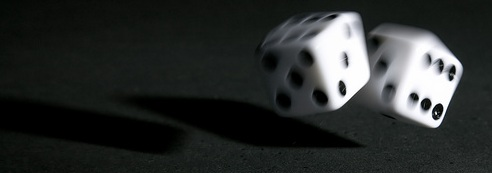
\includegraphics[width=3in]{dice.jpg}
\end{figure}
\FloatBarrier
}}

\begin{enumerate}

\easysubproblem{What brand name r.v. is $X_1$ distributed as? Write $X \sim$ something and make sure the parameters are correct. }\spc{1}

\easysubproblem{Does $X_1 \equalsindist X_2$? Yes or no is fine.}\spc{1}

\easysubproblem{Are $X_1$ and $X_2$ independent? Yes or no is fine.}\spc{1}

\easysubproblem{Compute $\expe{X_1}$ from first principles.}\spc{2}

\easysubproblem{Compute $\var{X_2}$ from first principles.}\spc{3}

\easysubproblem{The standard deviation is also called \qu{standard error} and it sometimes denoted \qu{SE.} Use your answer in (e) to find $\se{X_i}$  for $i \in \braces{1,2}$. Please just use the square root and do not rederive the variance again from scratch. }\spc{1}

\easysubproblem{Draw the PMF for $X_i$  for $i \in \braces{1,2}$ and mark $\expe{X_i}$ and $\se{X_i}$ on the graph similar to how we did in class.}\spc{6}

\easysubproblem{Imagine the game where you just double the winnings of a single roll. This would be equivalent to just multiplying the r.v. by a scale factor of 2. Calculate $\expe{2X_i}$, $\var{2X_i}$ and $\se{2X_i}$ from the formulas we learned in class. }\spc{3}

\easysubproblem{Draw the PMF for $2X_i$ for $i \in \braces{1,2}$ and mark $\expe{2X_i}$ and $\se{2X_i}$ that you calculated in (h) on the graph. }\spc{6}

\hardsubproblem{Draw the PMF for $X_1 + X_2$. This involves taking a convolution. Since convolution won't be on the midterm or final, I'm going to give a hint. There is 1 way to get 2 or 12, 2 ways to get 3 or 11, 3 ways to get 4 or 10, 4 ways to get 5 or 9, 5 ways to get 6 or 8 and 6 ways to get 7. }\spc{7}

\easysubproblem{Calculate $\expe{X_1 + X_2}$, $\var{X_1 + X_2}$ and $\se{X_1 + X_2}$ from the formulas we learned in class. Do not use the PMF from the last question; use the formulas from class.}\spc{2}

\hardsubproblem{Why are the standard errors in (h) and (k) different and why is (h) larger? This involves a lot of thinking and I want a few sentences \textit{in English}. }\spc{8}

\easysubproblem{Imagine the general case of $X_1, \ldots, X_n \iid$ with mean $\mu$ and variance $\sigsq$. Define $\Xbar$ as we did in class. Redo the derivation of $\expe{\Xbar} = \mu$.  }\spc{3}

\easysubproblem{Imagine the general case of $X_1, \ldots, X_n \iid$ with mean $\mu$ and variance $\sigsq$. Define $\Xbar$ as we did in class. Redo the derivation of $\se{\Xbar} = \sigma / \sqrt{n}$.  }\spc{3}


\hardsubproblem{Now you have the choice between game A --- where you roll $n$ times and average the winnings (\ie you collect $\Xbar_n$ dollars at the end) or game B --- where you roll one die and collect the amount you make on just one roll. Use your answers to the relevant previous questions (I won't tell you which ones explicitly) to explain why you would choose game A over B or vice versa. I want multiple sentences \textit{in English}. You must convince me you understand the tradeoff that game A and B are making.}\spc{5}


\intermediatesubproblem{Let $Z$ be the standardized r.v. for $\Xbar_n$. Standardization of a r.v. X is defined as subtracting its mean and dividing by its standard error. For $\Xbar$ this would be:

\beqn
Z := \frac{\Xbar - \expe{\Xbar}}{\se{\Xbar}} =\frac{\Xbar - \mu}{\frac{\sigma}{\sqrt{n}}}  
\eeqn

Prove from the formulas in class that $\expe{Z} = 0$ and $\var{Z} = \se{Z} = 1$. Hint: use those two rules about $\var{aX}$ and $\var{X + c}$ you just rederived}\spc{5}

\easysubproblem{Why is do you think \qu{standardization} is an appropriate term for what we did above?}\spc{2}


\intermediatesubproblem{Returning to $X$, the dice game in the beginning of the problem (the outcome results being \$1 if you roll a 1, \$2 if you roll a 2, \ldots, and \$6 if you roll a six), you calculated variance using the definition $\var{X} := \expe{\squared{X-\mu}}$ assuming the classic squared error loss: $e(x,\mu) := \squared{x - \mu}$. Imagine we defined a new variance metric using absolute loss, $e(x,\mu) := \abss{x - \mu}$. We'll denote this \qu{new variance} with a big squiggly symbol, $\widetilde{\var{X}} := \expe{\abss{X - \mu}}$ just to make sure you don't confuse it with the standard definition of $\var{X}$. Calculate $\widetilde{\var{X}}$ and include units.}\spc{10}

\end{enumerate}

\problem{More simple r.v. practice.}

\begin{enumerate}

\easysubproblem{You know that $T_n$ is the sum of $n$ $\iid$ bernoulli r.v.s with parameter $p$. Show that $\var{T_n}$ can be easily derived using the variance-sum formula we learned in class. }\spc{5}

\hardsubproblem{Show for any two r.v.'s $X$ and $Y$ which are independent that $\var{X \times Y} = \musq_X \sigsq_Y + \musq_Y \sigsq_X + \sigsq_X \sigsq_Y$. Remember, two r.v.'s multiplied together is a new r.v., $g(X, Y)$. }\spc{7}

\easysubproblem{Let $a_1, a_2, \ldots, a_n$ be a sequence of constants. Let $X_1, \ldots, X_n$ be a sequence of r.v.'s which thereby share the same mean $\mu$. Create a simplified expression for $\expe{a_1 X_1 + \ldots + a_n X_n}$. I want the simplest combination of symbols $a_1, a_2, \ldots, a_n$ and $\mu$. }\spc{4}

\intermediatesubproblem{Let $a_1, a_2, \ldots, a_n$ be a sequence of constants.  Assume $X_1, \ldots, X_n$ are a sequence of $\iid$ r.v.'s which thereby share the same variance $\sigsq$. Create a simplified expression for $\se{a_1 X_1 + \ldots + a_n X_n}$. I want the simplest combination of symbols $a_1, a_2, \ldots, a_n$ and $\mu$. }\spc{4}

\extracreditsubproblem{Imagine a r.v. $X$ with PMF $p(x) = c/x^2$ and $\support{X} = \naturals$. What is the exact value of $c$ which makes $p(x)$ a valid PMF? The answer can be found \href{http://en.wikipedia.org/wiki/Riemann_zeta_function}{here}. }\spc{3}

\extracreditsubproblem{$X$ is the same as in the previous problem. Show that $\var{X}$ does not exist (which means it's not a real number). You will need a fact from that same wikipedia page that you visited in the last problem. And now you've learned what the harmonic series is too. }\spc{10}

\end{enumerate}

\end{document}
